\chapter{Implementatie}

\section{Technologieën en software}

\subsection{Java 7}

Er zijn verschillende redenen waarom er gekozen is om de synchronisatie bibliotheek in Java te implementeren. De belangrijkste reden is dat de bestaande audio bibliotheken (Panako en TarsosDSP) van het IPEM ook ontwikkeld zijn in Java. Deze kunnen enkel aangeroepen worden via andere Java applicaties.

Het is ook de bedoeling is om de gebruikersinterface te ontwikkelen met behulp van Max/MSP modules. Het ontwikkelen van dergelijke modules is mogelijk in twee programmeertalen: C en Java. De eenvoud en hoge graad van abstractie gaf de doorslag om hierbij Java te gebruiken. De voordelen die C biedt op vlak van snelheid wegen (in deze toepassing) hier niet tegenop.

Hoewel de laatste versie van Max/MSP (7) het toelaat om Java 8 te gebruiken wordt deze versie in dit project om compatibiliteitsredenen vermeden. 

\subsection{JUnit}
JUnit is een unit testing framework voor Java. JUnit heeft in dit onderzoek een belangrijke rol gespeeld bij het bepalen van de optimale parameters van de verschillende algoritmen. JUnit maakte het mogelijk om de algoritmes herhaald maar met verschillende parameters op een dataset los te laten. JUnit liet toe om in één oogopslag te zien hoe het algoritme heeft gepresteerd.

\subsection{TarsosDSP}
\label{tarsos}

TarsosDSP is een Java bibliotheek voor realtime audio analyse en verwerking ontwikkeld aan het IPEM. De bibliotheek bevat een groot aantal algoritmes voor audioverwerking en kan nog verder worden uitgebreid. Deze bibliotheek wordt beschreven in artikel \cite{six2014tarsosdsp}. 

%Volgende paragraaf eventueel verplaatsen naar 3.5.1, ben er nog niet helemaal uit.
TarsosDSP is voornamelijk gebouwd rond het concept \textit{processing pipeline}. Dit is een abstractie van een audiostream die via programmacode verwerkt kan worden. Een processing pipeline wordt voorgesteld als instantie van de klasse \texttt{AudioDispatcher}. Een \texttt{AudioDispatcher} kan aangemaakt worden van een audiobestand, een array van floating-point getallen of een microfoon en kan bewerkt of verwerkt worden met behulp van één of meerdere \texttt{AudioProcessors}. Objecten van klassen die de interface \texttt{AudioProcessor} implementeren kunnen aan de processing pipeline worden toegevoegd. In de implementatie van de \texttt{process} methode kan de audiostream op een bepaalde manier verwerkt, geanalyseerd of gewijzigd worden.

TarsosDSP bevat verder nog een groot aantal klassen met allerhande tools en audioverwerkings algoritmen. Een greep uit de features van TarsosDSP:
\begin{itemize}[noitemsep]
	\item Toevoegen van geluidseffecten (delay, flanger,...)
	\item Toevoegen van filters (low-pass, high-pass, band-pass,...)
	\item Conversie tussen verschillende formaten
	\item Toonhoogte detectie
	\item Wijzigen van de samplefrequentie
\end{itemize}

\subsection{Panako}

Panako is net zoals TarsosDSP een Java bibliotheek (door de zelfde auteur) ontwikkeld aan het IPEM. Panako bevat een arsenaal aan algoritmen voor het matchen of synchroniseren van audiofragmenten of audiostreams.  Deze bibliotheek wordt uitgebreid beschreven in artikel \cite{six2014panako}.

Dit onderzoek gebruikt Panako's open-source implementatie van het acoustic fingerprinting algoritme dat beschreven is in artikel \cite{Wang2003a}. Panako bevat ook een uitbreiding van het algoritme dat overweg kan met audio waarbij de toonhoogte verhoogd of verlaagd is, of waarbij de audio sneller of trager is afgespeeld.

Buiten het algoritme bevat de bibliotheek ook verschillende toepassingen die hiervan gebruik maken. Zo is het mogelijk om de fingerprints van een geluidsfragment te bekijken, matches tussen verschillende geluidsfragmenten te visualiseren, en grafisch te experimenteren met de verschillende parameters. Figuur \ref{fingerprint_visualiser} toont een screenshot van deze toepassing.

\begin{figure}[!h]
	\captionsetup{width=0.8\textwidth}
	\caption[Gebruikersinterface van Audacity]{De gebruikersinterface van Panako's NFFT Fingerprint Visualiser. Onderaan kunnen de parameters van het algoritme met behulp van sliders gewijzigd worden.}
	\centering
	\advance\parskip0.3cm
	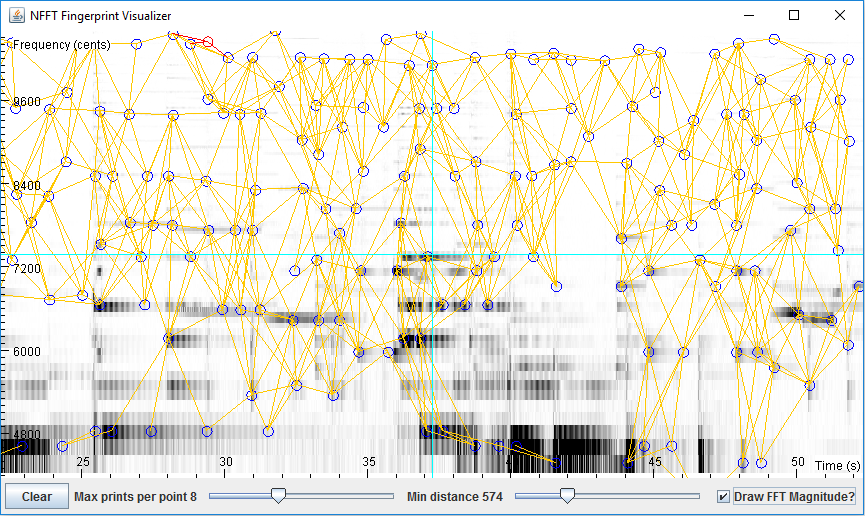
\includegraphics[width=0.8\textwidth]{fingerprint_visualiser.png}
	\label{fingerprint_visualiser}
\end{figure}

Er is ook een applicatie beschikbaar (SyncSink) om verschillende geluidsfragmenten te synchroniseren. Deze applicatie gebruikt naast het acoustic fingerprinting algoritme ook het kruiscovariantie algoritme. 

Na het bepalen van de latency tussen de verschillende audiofragmenten kan de applicatie een shell script genereren dat met behulp van \textit{FFmpeg} stukjes van de geluidsbestanden wegknipt of er stilte aan toevoegt. Het resultaat is dat na het uitvoeren van het script de geluidsbestanden gesynchroniseerd zijn.

\subsection{FFmpeg}

FFmpeg is een command-line multimedia framework dat gebruikt wordt voor encoderen, decoderen, multiplexen, demultiplexen, streamen en afspelen van audio en video. \cite{kollarconfiguration}

In dit onderzoek wordt FFmpeg voornamelijk gebruikt in scripts bij het geautomatiseerd genereren van testdata.

\subsection{SoX}

SoX is net zoals FFmeg een command-line tool voor audioverwerking. Buiten de mogelijkheid om audiobestanden te converteren laat SoX ook minder triviale operaties toe. Zo is het onder meer mogelijk om het volume aan te passen, effecten toe te voegen, de bestanden bij te knippen of gegenereerde geluiden in een audiobestand te mixen.
\cite{barras2012sox}

In dit onderzoek wordt SoX gebruikt in scripts bij het manipuleren van de testdata.

\subsection{Sonic Visualiser}

Sonic Visualiser is een gebruiksvriendelijke desktopapplicatie voor de analyse, visualisatie van audiobestanden. Sonic Visualiser laat toe om audiobestanden vanuit verschillende perspectieven te analyseren. Zo kan zowel de golfvorm als het spectrogram van een audiobestand gevisualiseerd worden. Sonic Visualiser is uitbreidbaar met plug-ins in het \textit{Vamp} formaat. \cite{cannam2010sonic}

\begin{figure}[!h]
	\captionsetup{width=0.8\textwidth}
	\caption[Gebruikersinterface van Sonic Visualiser]{De gebruikersinterface van Sonic Visualiser}
	\advance\parskip0.3cm
	\centering
	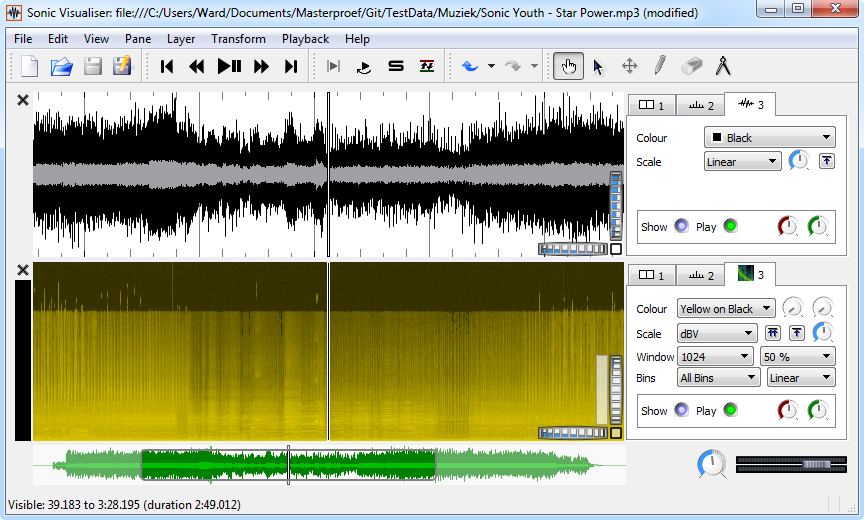
\includegraphics[width=0.8\textwidth]{sonicvisualiser.png}
\end{figure}

Sonic Visualiser werd in dit onderzoek vooral gebruikt als testtool om handmatig de latency tussen verschillende audiofragmenten te bepalen. De handmatig bepaalde latency werd vervolgens vergeleken met de berekende resultaten.

\subsection{Audacity}

Audacity is een open-source desktopapplicatie voor het bewerken, opnemen en converteren van audio. Met Audacity is het ook mogelijk om tal van effecten en filters aan audio toe te voegen.\cite{audacity2016} 

Figuur \ref{screenshot-audacity} toont de gebruikersinterface van dit programma.

\begin{figure}[!h]
	\captionsetup{width=0.8\textwidth}
	\caption[Gebruikersinterface van Audacity]{De gebruikersinterface van Audacity}
	\centering
	\advance\parskip0.3cm
	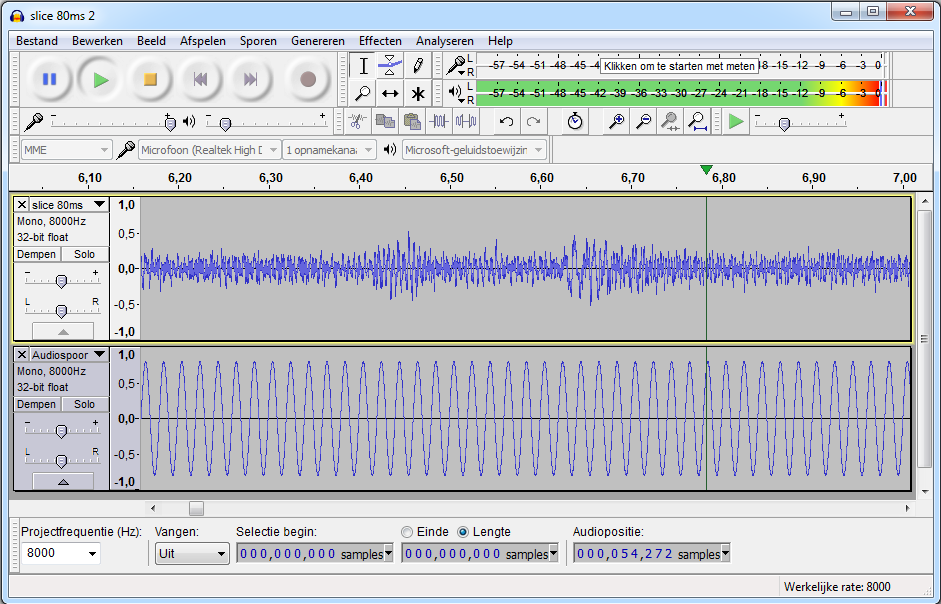
\includegraphics[width=0.8\textwidth]{audacity.png}
	\label{screenshot-audacity}
\end{figure}

Alle opnames en handmatige bewerkingen op audiobestanden in dit onderzoek zijn uitgevoerd met behulp van Audacity. 

\subsection{Max/MSP}

Max/MSP is een visuele programmeertaal voor muziek en multimedia. Het is een systeem waarbij modules met elkaar verbonden kunnen worden om zo complexere systemen op te bouwen. Max/MSP beschikt ook over een API waarmee in Java of C nieuwe modules ontwikkeld kunnen worden. \cite{cycling2016}

\begin{figure}[!h]
	\captionsetup{width=0.8\textwidth}
	\caption[Gebruikersinterface van Max/MSP]{De gebruikersinterface van Max/MSP: een \textit{patch panel} met daarop enkele modules die samen een complexere toepassing vormen.}
	\centering
	\advance\parskip0.3cm
	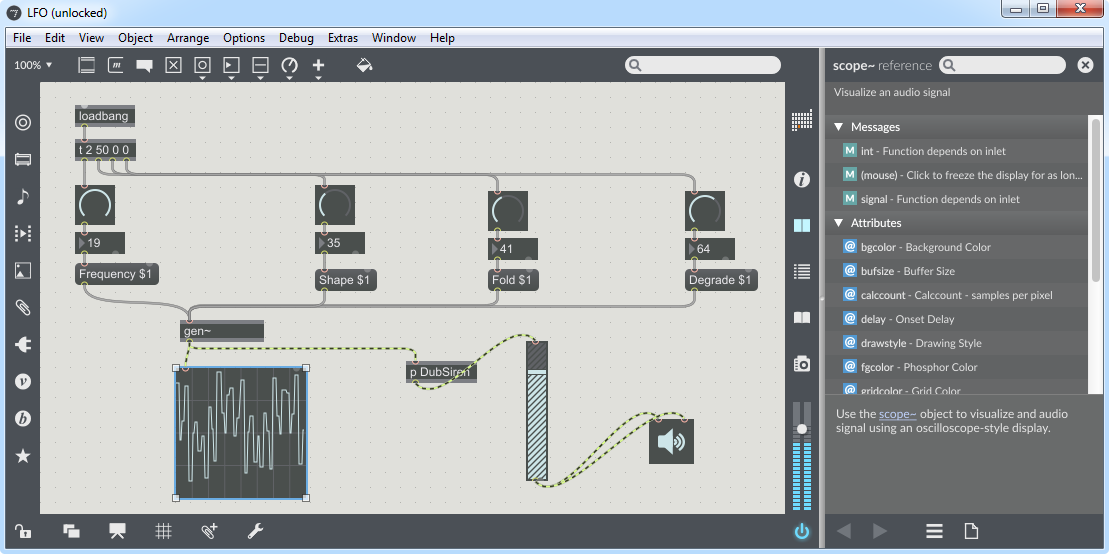
\includegraphics[width=0.8\textwidth]{maxmsp.png}
	\label{screenshot-max}
\end{figure}

Met Max/MSP is het mogelijk om realtime audio te  verwerken, daarom zal deze toepassing gebruikt worden voor het ontwikkelen van de gebruikersinterface. 

Figuur \ref{screenshot-max} toont een eenvoudige Max/MSP patch.

\subsection{Teensy}

De Teensy is een kleine microcontroller die via USB geprogrammeerd kan worden. De Teensy is compatibel met de Arduino software en is hierdoor zeer gebruiksvriendelijk. \cite{teensy2016}

De sensoren die gebruikt worden bij de experimenten van het IPEM zijn meestal aangesloten op Teensy microcontrollers.

\begin{figure}[!h]
	\captionsetup{width=0.7\textwidth}
	\caption[Teensy microcontroller]{De Teensy microcontroller verbonden met een infraroodsensor en microfoon op een breadboard.}
	\centering
	\advance\parskip0.3cm
	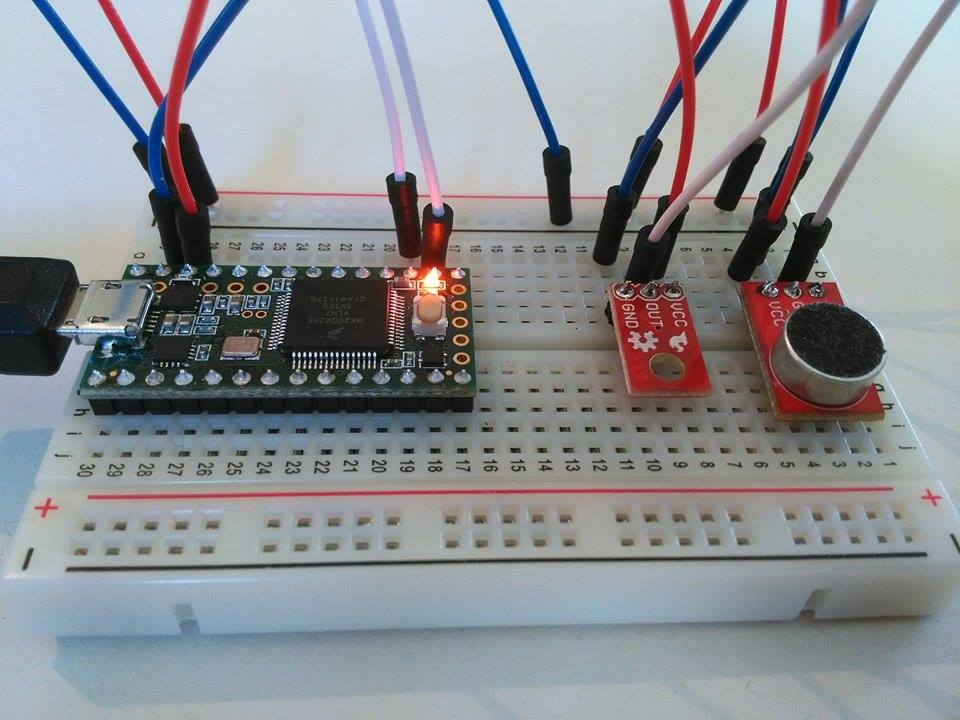
\includegraphics[width=0.4\textwidth]{teensy.jpg}
	\label{teensy-pic}
\end{figure}

In hoofdstuk \ref{evaluatie} worden de testen die met de Teensy microcontroller zijn uitgevoerd meer in detail besproken. Figuur \ref{teensy-pic} toont een typische testopstelling waarbij twee sensoren zijn aangesloten op de microcontroller.

\section{Acoustic fingerprinting}

De Panako softwarebibliotheek bevat een implementatie van het acoustic fingerprinting algoritme. Om wijzigingen mogelijk te maken hebben is de code van het algoritme overgenomen in het project van dit onderzoek. De aangepaste code blijft wel nog steeds afhankelijk van enkele klassen uit het Panako project. 

\subsection{Optimalisaties}

Aan dit algoritme is één vereenvoudiging aangebracht. Het originele algoritme bevatte namelijk de mogelijkheid om alle offsets boven een bepaalde drempelwaarde te verwerken. Deze feature laat toe dat er meerdere matches kunnen gevonden worden binnen één uitvoering van het algoritme. Om dit te ondersteunen moeten alle matches echter wel één voor één worden vergeleken met de drempelwaarde. Omdat deze toepassing enkel de beste offsetwaarde nodig heeft is dit overbodig. De beste offset en bijhorende fingerprints wordt apart bijgehouden. Hierbij wordt vermeden dat de matches op het einde moeten worden overlopen.

\subsection{Parameters en hun invloed op het algoritme}
\label{acoustic-fingerprinting-params}

De werking van dit algoritme is afhankelijk van een aantal parameters die een grote invloed kunnen hebben op de performantie en de nauwkeurigheid van het uiteindelijke resultaat. Daarom is het van belang om voor het uitvoeren van het algoritme de waarde van deze parameters te controleren. De optimale waarde van elke parameter is afhankelijk van verschillende factoren die van situatie tot situatie kunnen verschillen:

\begin{itemize}[noitemsep]
\item de vereiste nauwkeurigheid van het algoritme;
\item de vereiste performantie van het algoritme;
\item de mate waarin er omgevingsgeluid aanwezig is;
\item de opnamekwaliteit van het omgevingsgeluid.
\end{itemize}

De meeste parameters worden bijgehouden in een configuratiebestand waardoor ze ook na compilatie wijzigbaar zijn. Dit zijn de belangrijkste parameters uit het configuratiebestand die invloed hebben op het algoritme:

\begin{description}
\item\texttt{SAMPLE\_RATE} \hfill \\
Deze parameter bepaalt de standaard samplefrequentie die gebruikt wordt tijdens het synchronisatieproces. Het verhogen van deze parameter zorgt voor een tragere verwerking maar een betere nauwkeurigheid. Afhankelijk van op welke manier de synchronisatie wordt opgestart (via Max of met een \texttt{AudioDispatcher}) worden de binnenkomende streams geresamplet of wordt al een correcte samplefrequentie verondersteld.

\item\texttt{NFFT\_BUFFER\_SIZE}\footnote{De letter N in NFFT heeft geen noemenswaardige betekenis. De naam is overgenomen van de gelijknamige parameter uit de Panako bibliotheek.} \hfill \\
Dit is de grootte van de verschuivende buffer die gebruikt wordt in het FFT algoritme. Deze parameter is cruciaal aangezien de frequentiesterktes op een bepaalde plaats op de tijd\-as worden berekend per buffer. Deze parameter wordt uitgedrukt in aantal samples.
\item\texttt{NFFT\_STEP\_SIZE} \hfill \\
Dit is het aantal samples van elke verschuiving in het FFT algoritme. De stepsize beïnvloedt rechtstreeks de nauwkeurigheid van het acoustic fingerprinting algoritme. Wanneer deze parameter is ingesteld op 128 samples en een samplefrequentie van 8000hz dan is de maximale nauwkeurigheid $128/8000Hz = 0.016s = 16ms$.
\item\texttt{MIN\_ALIGNED\_MATCHES} \hfill \\
Een match tussen twee audiofragmenten wordt pas als geldig beschouwd wanneer er een bepaald aantal matchende fingerprints met dezelfde offset gevonden zijn. Dit aantal wordt ingesteld met deze parameter.
\item\texttt{NFFT\_MAX\_FINGERPRINTS\_PER\_EVENT\_POINT} \hfill \\
Deze parameter bepaalt het maximum aantal fingerprints waaraan een event point (een punt op het spectrogram) kan deelnemen. Hoe hoger dit maximum hoe vlugger er matches kunnen gevonden worden. Het hanteren van een hoge waarde heeft een negatieve invloed op de performantie.
\item\texttt{NFFT\_EVENT\_POINT\_MIN\_DISTANCE} \hfill \\
Dit is de minimale afstand tussen twee event points op het spectrogram die samen een fingerprint kunnen vormen. 

\end{description}

Verder maakt het algoritme nog gebruik van twee hardgecodeerde parameters die niet instelbaar zijn via het configuratiebestand: \texttt{MIN\_FREQUENCY} en \texttt{MAX\_FREQUENCY}. Deze parameters bepalen binnen welke frequentiebereik er naar fingerprints gezocht worden. De waarden waarop deze ingesteld staan bevinden zich op de rand van de frequenties die door muziek of stemgeluid geproduceerd worden.

\subsection{Optimale instellingen}
\label{optimal-acoustic-fingerprinting}

Het bepalen van de optimale waarden voor de parameters is geen exacte wetenschap maar eerder een probleem dat proefondervindelijk moet worden aangepakt.

Bij het acoustic fingerprinting algoritme is er een groot verschil tussen de meest ``elegante'' parameterwaarden en de in de praktijk best presterende waarden. Dit verschil zal duidelijk worden in volgende opsomming waarin elke parameter zal worden besproken.


\begin{description}
	\item\texttt{SAMPLE\_RATE} \hfill \\
	Bij deze parameter is het van belang om een goede balans te vinden zodat de geluidskwaliteit aanvaardbaar blijft zonder een hypotheek te plaatsen op de performantie van het algoritme. De praktijk heeft uitgewezen dat bij een samplefrequentie van $ 8000Hz $ het algoritme goed presteert. Deze waarde wordt bevestigd in artikel \cite{six2015multimodal}.
	\item\texttt{NFFT\_BUFFER\_SIZE} en \texttt{NFFT\_STEP\_SIZE} \hfill \\
	De ingesteld waarden van de samplefrequentie, buffergrootte en stapgrootte zijn afhankelijk van elkaar. Om een goede werking van het FFT algoritme te garanderen bij een samplefrequentie van $ 8000Hz $ worden de buffergrootte en stapgrootte respectievelijk ingesteld op 512 en 128 (of 256) samples. Deze waarden worden eveneens vermeld in artikel \cite{six2015multimodal}.
	\item\texttt{MIN\_ALIGNED\_MATCHES} \hfill \\
	In een toepassing zoals het detecteren van liedjes ten opzichte van een database is het secuur instellen van deze parameter erg belangrijk. Deze parameter heeft namelijk een grote invloed op het voorkomen van \textit{false positives} of \textit{false negatives}. 
	
	Bij het synchroniseren van streams is de situatie echter helemaal anders. Het binnenkrijgen van een false positive (=foute latency) is veel minder erg dan het helemaal niet binnenkrijgen van (mogelijk correcte) resultaten. Aangezien het algoritme per buffer enkel het beste resultaat teruggeeft is de kans dat bij geluidsfragmenten van behoorlijke kwaliteit eenzelfde foute latency meer voorkomt dan de correcte latency zéér klein.
	
	Bij geluidsfragmenten van mindere kwaliteit kan het gebeuren dat er toch foute resultaten door de mazen van het net glippen. Om dit te vermijden is het mogelijk om nog een extra filtering toe te passen. In deze extra stap worden eventuele uitschieters geëlimineerd.
	
	Bovenstaande argumenten stellen duidelijk dat het beter is om deze parameter een lage waarde te geven. In deze toepassing is gekozen voor de waarde 2 in plaats van het absolute minimum 1: hierdoor wordt pure willekeur bij het matchen van audiofragmenten van extreem slechte kwaliteit vermeden. Dit is laag in vergelijking met Panako waar 7 de standaard waarde is van deze parameter.
	
	\item\texttt{NFFT\_MAX\_FINGERPRINTS\_PER\_EVENT\_POINT} \hfill \\
	In Panako is het standaard dat een event point uitmaakt van maximaal 2 fingerprints. Het hanteren van deze waarde leidt ertoe dat het matchen van audiofragmenten van behoorlijke kwaliteit zeer snel kan worden uitgevoerd. 
	
	In deze toepassing is het aantal te vergelijken audiofragmenten meestal erg beperkt. Ook is de kwaliteit van deze fragmenten vaak van ondermaats (bv. de opnames op microcontrollers). Daarom is het in dit geval een goed idee om de waarde van deze parameter zéér hoog in te stellen. Hierdoor verhoogt de kans sterk dat er bij zeer slechte audiofragmenten toch enkele overeenkomende fingerprints gevonden worden. Testen hebben uitgewezen dat de negatieve invloed op de performantie beperkt blijft en dat de resultaten sterk verbeteren. 
	
	Bij het zoeken naar matches tussen geluidsopnames opgenomen op microcontrollers heeft de praktijk uitgewezen dat het toelaten van maximaal 50 fingerprints per event point degelijke resultaten oplevert.
	%TODO: refereren naar testresultaen
	
	\item\texttt{NFFT\_EVENT\_POINT\_MIN\_DISTANCE} \hfill \\
	In tegenstelling tot vorige parameter zorgt het verhogen van deze waarde ervoor dat er minder fingerprints worden gecreëerd. De argumenten die bij vorige parameter zijn aangehaald gelden bijgevolg in omgekeerde zin ook voor deze parameter. Hoewel de Panako standaard 600 is leveren waardes rond het getal 20 in deze toepassing de beste resultaten zonder de performantie sterk te beperken.
	
	
\end{description}


\section{Kruiscovariantie}

De Panako bibliotheek bevatte bij aanvang van dit onderzoek al een implementatie van het kruiscovariantie algoritme. In tegenstelling tot het acoustic fingerprinting algoritme was het echter minder grondig afgewerkt. Om degelijke resultaten te garanderen was het noodzakelijk om enkele anomalieën in de geleverde resultaten te analyseren en de oorzaak hiervan op te lossen. Om te kunnen begrijpen wat er precies fout ging moet eerst de integratie met het acoustic fingerprinting algoritme besproken worden.

Net zoals het acoustic fingerprinting algoritme is de code overgenomen in het project van dit onderzoek. De code is niet meer afhankelijk van de Panako bibliotheek.

\subsection{Integratie met acoustic fingerprinting}
\label{integratie-acoustic-fingerprinting}

In sectie \ref{toepasbaarheid} is er geschreven dat de latency zeer nauwkeurig kan bepaald worden door het berekenen van de kruiscovariantie. Vanwege de performantie is het wel noodzakelijk om eerst de ruwe latency met acoustic fingerprinting te bepalen. Hoe deze algoritmes geïntegreerd worden zal hier worden besproken. 

Onderstel twee geluidsopnames: de tweede opname heeft een vertraging van 90 ms ten opzichte van de eerste referentieopname. Het uitvoeren van het acoustic fingerprinting algoritme met standaard parameters (tot op $ 32 ms $ nauwkeurig) kan twee resultaten opleveren: $ 64 ms $ of $ 96 ms $. Na het berekenen van de kruiscovariantie kan bepaald worden of er zich een onderschatting (eerste waarde) of overschatting (tweede waarde) heeft voorgedaan, dit is van belang om het resultaat correct te verfijnen. Figuur \ref{crosscovariance1} toont de mogelijke resultaten van het algoritme.

Als de ruw bepaalde latency positief is wordt deze waarde van het tweede fragment weggeknipt. Na deze stap is de latency tussen de resterende audiofragmenten zeker minder dan de minimale nauwkeurigheid van het acoustic fingerprinting algoritme. 

\begin{figure}[h!]
	\captionsetup{width=0.7\textwidth}
	\caption[Kruiscovariantie audiofragmenten]{Twee audiofragmenten: het tweede audiofragment heeft een latency van 90 milliseconden ten opzichte van het eerste.}
	\begin{center}
		\advance\parskip0.3cm
		\begin{tikzpicture}[scale=1]
\begin{axis}[
xlabel={Tijd (milliseconden)},
xmin=0,xmax=500,
ymin=0,ymax=1,
legend style={
	cells={anchor=west},
	legend pos=outer north east,
},
yticklabels={,,},
xticklabel style={grid=major},
extra x ticks ={64,90,96},
extra x tick labels={,,,},
extra tick style={grid=major, grid style={dotted}},
hide y axis
]

\addplot[thick,black] graphics[xmin=0,ymin=0.5,xmax=500,ymax=0.8] {reference.png};

\addplot[thick,black] graphics[xmin=0,ymin=0.0,xmax=500,ymax=0.3] {other.png};


after end axis/.code={

	
	\draw[black,<->] (axis cs:0,0.42) -- (axis cs:96,0.42)	node [pos=0.5,above,font=\scriptsize] {$96ms$};
	
	\draw[black,<->] (axis cs:0,0.32) -- (axis cs:90,0.32)	node [pos=0.5,above,font=\scriptsize] {$90ms$};
	
	\draw[black,<->] (axis cs:0,0.22) -- (axis cs:64,0.22)	node [pos=0.5,above,font=\scriptsize] {$64ms$};
}]

\node at (axis cs:250,0.82) [] {Referentie};
\node at (axis cs:250,0.35) [] {Andere};

\end{axis}

\end{tikzpicture}
	\end{center}
	\label{crosscovariance1}
\end{figure}


Vervolgens worden een aantal samples van elk audiofragment gekopieerd naar een buffer. De latency tussen deze twee buffers wordt berekend met het kruiscovariantie algoritme (beschreven in sectie \ref{kruiscovariantie}). Figuur \ref{crosscovariance2} toont de buffers waarop het algoritme kan worden uitgevoerd bij een buffergrootte van 512 samples en samplefrequentie van $ 8000Hz $.

\begin{figure}[h!]
	\captionsetup{width=0.7\textwidth}
	\caption[Kruiscovariantie buffers]{Kruiscovariantie buffers na het wegknippen van de $ 96 ms $ latency bepaald door het acoustic fingerprinting algoritme. Hier heeft de referentie audio $ 6 ms $ latency ten opzichte van het andere audiofragment.   }
	\begin{center}
		\advance\parskip0.3cm
		\begin{tikzpicture}[scale=1]
\begin{axis}[
xlabel={Tijd (milliseconden)},
xmin=0,xmax=64,
ymin=0,ymax=1,
legend style={
	cells={anchor=west},
	legend pos=outer north east,
},
yticklabels={,,},
xticklabel style={grid=major},
%extra x ticks ={64,90,96},
extra x tick labels={,,,},
extra tick style={grid=major, grid style={dotted}},
hide y axis,
width = 15cm,
height = 7cm
]

\addplot[thick,black] graphics[xmin=0,ymin=0.6,xmax=64,ymax=0.9] {refcut.png};

\addplot[thick,black] graphics[xmin=0,ymin=0.1,xmax=64,ymax=0.4] {othercut.png};


after end axis/.code={
	\draw[black,<->] (axis cs:0,0.85) -- (axis cs:6,0.85)	node [pos=0.5,above,font=\scriptsize] {$6ms$};
}]

\node at (axis cs:32,0.85) [] {Referentie};
\node at (axis cs:32,0.37) [] {Andere};

\end{axis}

\end{tikzpicture}
	\end{center}
	\label{crosscovariance2}
\end{figure}

Wanneer het acoustic fingerprinting algoritme de werkelijke latency heeft onderschat wordt de verfijnde latency bekomen door de ruwe latency en het resultaat van het kruiscovariantie algoritme op te tellen. Bij een overschatting is dit niet het geval.

Aangezien het kruiscovariantie algoritme de latency zoekt van de ``andere'' buffer ten opzichte van de referentiebuffer zal het resultaat niet $6 ms$ maar $ 58 ms $ zijn. Dit komt doordat het algoritme de ``andere'' buffer cyclisch (maar in de verkeerde zin) verschuift.

Om in een dergelijke situatie de verfijnde latency te berekenen moet men van de som van de resultaten ($96 ms + 58 ms$) nog de lengte van de gebruikte buffer ($ 64ms $) aftrekken. De verfijnde latency is dus $ 154 ms - 64 ms = 90 ms $.

%Eventueel nog schrijven hoe bepaald wordt of het resultaat onderschat of overschat is.

\subsection{Optimalisaties}

\subsubsection{Bugfixes}

In de originele versie van het algoritme werd geen rekening gehouden met het feit dat het acoustic fingerprinting algoritme het de werkelijke latency kan overschatten of onderschatten. De latency bepaalt door het kruiscovariantie algoritme werd telkens opgeteld bij de ruwe latency bepaald door het acoustic fingerprinting algoritme. In 50\% van de gevallen leidde dit probleem tot foutieve resultaten.

\subsubsection{Meerdere malen uitvoeren van het algoritme}
\label{crosscovariance-repeated}

In tegenstelling tot acoustic fingerprinting is het bepalen van de latency met kruiscovariantie veel meer foutgevoelig. Bij opnames van slechte kwaliteit worden vaak foute resultaten teruggegeven. 

Hoewel bij acoustic fingerprinting mogelijk storende factoren (een zoemende toon, geruis,...) zichtbaar zijn in het spectrogram zullen er naar alle waarschijnlijkheid nog steeds voldoende fingerprints gegenereerd worden op basis van geluiden die wel in beide opnames voorkomen. 

\begin{figure}[h!]
	\captionsetup{width=0.7\textwidth}
	\caption[Zoemtoon van $50 Hz$]{Twee gelijke audiofragmenten. Aan het tweede audiofragment is een achtergrondtoon van $50 Hz$ toegevoegd.}
	\begin{center}
		\advance\parskip0.3cm
		\begin{tikzpicture}[scale=1]
\begin{axis}[
xlabel={Tijd (milliseconden)},
xmin=0,xmax=140,
ymin=0,ymax=1,
legend style={
	cells={anchor=west},
	legend pos=outer north east,
},
yticklabels={,,},
xticklabel style={grid=none},
extra x tick labels={,,,},
extra tick style={grid=major, grid style={dotted}},
hide y axis,
width = 15cm,
height = 6cm
]

\addplot[thick,black] graphics[xmin=0,ymin=0.6,xmax=140,ymax=0.9] {zoemtoon-origineel.png};

\addplot[thick,black] graphics[xmin=0,ymin=0.1,xmax=140,ymax=0.4] {zoemtoon.png};


after end axis/.code={
%	\draw[black,<->] (axis cs:0,0.85) -- (axis cs:6,0.85)	node [pos=0.5,above,font=\scriptsize] {$6ms$};
}]

\node at (axis cs:70,0.88) [] {Origineel fragment};
\node at (axis cs:70,0.40) [] {Fragment met $50 Hz$ toon};

\end{axis}

\end{tikzpicture}
	\end{center}
	\label{zoemtoon}
\end{figure}

Dergelijke storende elementen hebben veel meer invloed op het kruiscovariantie algoritme. Een ongewenste zoemende bastoon zorgt voor een grote verandering van de geluidsgolf van het audiofragment. Aangezien de kruiscovariantie rechtstreeks tussen twee geluidsgolven berekent wordt kan dit serieuze gevolgen hebben. In figuur \ref{zoemtoon} wordt dit probleem visueel verduidelijkt.

De invloed van storende factoren zoals zoemende tonen en ruis is gemakkelijk te beperken. Aangezien het kruiscovariantie algoritme over een zéér klein deeltje van het audiofragment wordt uitgevoerd is het zeer eenvoudig om het algoritme tientallen keren, maar telkens op een andere plaats, uit te voeren. Na elke iteratie wordt de latency in het geheugen opgeslagen. Ten slotte wordt er gezocht naar de latency die het meeste voorkomt. Die latency wordt gebruikt om het resultaat van het acoustic fingerprinting algoritme te verfijnen.

\subsection{Parameters en hun invloed op het algoritme}

De parameters van het kruiscovariantie algoritme zijn net zoals die van het acoustic fingerprinting algoritme instelbaar via het configuratiebestand.

\begin{description}	
	\item\texttt{NFFT\_BUFFER\_SIZE} \hfill \\
	Hoewel het FFT algoritme eigenlijk niets te maken heeft met het berekenen van de kruiscovariantie speelt deze parameter bij dit algoritme toch een belangrijk rol. Deze parameter bepaalt namelijk de grootte van de buffers waartussen de kruiscovariantie berekent wordt. Om een goede werking van het kruiscovariantie algoritme te verzekeren is het een vereiste dat de gebruikte buffers groter zijn dan de minimale nauwkeurigheid van het acoustic fingerprinting algoritme (anders is het mogelijk dat na het knippen de audiofragmenten er geen gelijkenissen te vinden zijn tussen beide buffers). Aangezien deze nauwkeurigheid bepaald wordt de \texttt{NFFT\_STEP\_SIZE} parameter en de \texttt{NFFT\_BUFFER\_SIZE} hier altijd een veelvoud van is, is het gemakkelijk om deze parameter ook voor het kruiscovariantie algoritme te gebruiken.
	
	\item\texttt{CROSS\_COVARIANCE\_NUMBER\_OF\_TESTS} \hfill \\
	Deze parameter bepaalt het aantal keren dat het kruiscovariantie algoritme per slice (zie \ref{streambuffers}) zal worden uitgevoerd. De meest voorkomende latency wordt als resultaat teruggegeven.
	
	\item\texttt{CROSS\_COVARIANCE\_THRESHOLD} \hfill \\
	Deze parameter bepaalt het minimum aantal keer dat een latency moet voorkomen om als geldig beschouwd te mogen worden.	Stel dat het algoritme 50 keer wordt uitgevoerd maar elke keer een verschillend resultaat teruggeeft, dan zal er geen latency worden teruggegeven indien deze parameter staat ingesteld op een waarde groter dan 1.
	
\end{description}

\subsection{Optimale instellingen}
\begin{description}	
	\item\texttt{NFFT\_BUFFER\_SIZE} \hfill \\
	De optimale waarde van deze parameter werd in sectie \ref{optimal-acoustic-fingerprinting} besproken.
	
	\item\texttt{CROSS\_COVARIANCE\_NUMBER\_OF\_TESTS} \hfill \\
	Bij audiofragmenten van goede kwaliteit is het niet noodzakelijk om deze parameter een hoge waarde te geven. Als het algoritme 5 à 10 keer wordt uitgevoerd zal de correcte latency hoogst waarschijnlijk al verschillende malen gevonden zijn. 
	
	Bij audiofragmenten van slechte kwaliteit is het van belang om deze parameter zo hoog mogelijk in te stellen. Aangezien het kruiscovariantie algoritme vrij intensief is hangt de waarde wat af van de beschikbare rekenkracht. De praktijk heeft uitgewezen dat de waarde 50 een goed evenwicht biedt tussen correctheid en performantie.
	
	Deze parameter heeft als bovengrens ($ N_B $) het aantal keren dat een kruiscovariantie buffer (bepaald door \texttt{NFFT\_BUFFER\_SIZE}) past in een streambuffer (zie \ref{streambuffers}) waarin de streams worden ingelezen (bepaald door \texttt{SLICE\_SIZE\_S}). Dit kan worden berekend met volgende formule:
	\begin{equation}
		N_B = \frac{\texttt{SLICE\_SIZE\_S}}{\texttt{NFFT\_BUFFER\_SIZE} \cdot \texttt{SAMPLE\_RATE}}
	\end{equation}
	
	\item\texttt{CROSS\_COVARIANCE\_THRESHOLD} \hfill \\
	Het hoog instellen van deze waarde heeft enkel nut als het van belang is dat het kruiscovariantie algoritme zeker een correct resultaat teruggeeft. In de huidige implementatie wordt het ruwe resultaat gebruikt als het aantal gelijke waarden niet boven deze drempel komt. Daarom wordt deze waarde meestal op 1 ingesteld. De best mogelijke verfijning van het resultaat wordt dan toegepast, ongeacht het aantal keer dat het resultaat voorkomt. 
\end{description}

\section{Filteren van de resultaten}
\label{filtering}

Het is moeilijk om met zekerheid te bepalen of een bepaalde latency correct is. Toch kan er een soort van statistische optimalisatie worden uitgevoerd op de opeenvolgende latencies. De kans is namelijk klein dat de werkelijke latency verandert en na een korte tijd terugkeert naar de originele waarde.\footnote{Theoretisch is een dergelijke situatie toch mogelijk: In dit voorbeeld wordt de latency bepaalt tussen de audiostreams ($ 8000 Hz$ samplefrequentie) van twee Teensy microcontrollers. Wanneer er 50 samples gedropt worden van de referentie audiostream zorgt dit voor een latencyverhoging van de andere audiostream van $6 ms$. Indien er enkele seconden later 50 samples gedropt worden van de andere audiostream dan leidt dit tot een vermindering van de latency van $ 6 ms $. Visueel is dit een piek in de opeenvolgende latencies.} Ook is de kans klein dat een foute latency toevallig verschillende malen na elkaar gedetecteerd wordt.

Deze eigenschappen laten toe om toch een bepaalde vorm van ``foutherstelling'' te implementeren. Fouten kunnen namelijk weggefilterd worden door eventuele pieken in opeenvolgende latencies af te vlakken.

\subsection{Werking}

Het afvlakken van pieken kan in realtime geïmplementeerd worden door gebruik te maken van verschillende \textit{sliding windows}. Per audiostream wordt een buffer bijgehouden met daarin de opeenvolgende latencies ten opzichte van de referentie audiostream. Wanneer een buffer haar maximumcapaciteit heeft bereikt gaat het toevoegen van een nieuwe latency gepaard met het verwijderen van de oudste latency.

Het afvlakken van pieken wordt verwezenlijkt door in plaats van de meest recente latency het gemiddelde of de mediaan van de buffer te gebruiken. De mate waarin pieken worden afgevlakt hangt af van de grootte van de buffer en de gebruikte methode (gemiddelde of mediaan).

\subsection{Voorbeelden}

De effectiviteit van de verschillende parameters (buffergrootte en filtermethode) zal in dit gedeelte worden weergegeven aan de hand van enkele voorbeelden. Er zullen verschillende soorten filters worden toegepast op een verloop van 35 latencies. In het ongefilterde verloop (zie figuur \ref{latencydata}) komen twee grote en drie kleine (waarschijnlijk foutieve) pieken voor. Na het vijftiende resultaat doet er zich een blijvende (correcte) verhoging van de latency voor.

\newcommand{\datafiltergraph}[1]
{
	\begin{tikzpicture}[scale=0.9]
		\begin{axis}[
		ylabel={Latency (ms)},
		xtick ={0,5,10,15,...,35},
		ytick ={60,80,...,180},
		ymin = 60,
		ymax = 180,
		height = 5cm,
		width = 8cm
		]
		\addplot [mark=none] table {#1.dat};
		\end{axis}
	\end{tikzpicture}
}


\begin{figure}[h!]
	\captionsetup{width=0.7\textwidth}
	\caption[Het ongefilterde verloop van de latency]{Grafische weergave van het ongefilterde verloop van de latency.}
	\begin{center}
		\advance\parskip0.3cm
		\datafiltergraph{latencydata}
	\end{center}
	\label{latencydata}
\end{figure}

\subsubsection{Moving average filter}

De eerste twee voorbeelden tonen het verschil tussen de ongefilterde latencies en de latencies die gefilterd zijn door het gemiddelde van een buffer te nemen. Bij het eerste voorbeeld bevat de buffer maximum 3 latencies, bij het tweede voorbeeld kan de buffer maximum 5 latencies bevatten.

\begin{figure}[!tbph]
	\centering
	\subfloat[Buffergrootte 3]{\datafiltergraph{avg3data}}
	\hfill
	\subfloat[Buffergrootte 5]{\datafiltergraph{avg5data}}
	\captionsetup{width=0.7\textwidth}
	\caption{Het verloop van de latencies na het toepassen van een moving average filter.}
\end{figure}

Ondanks het toepassen van de filter blijven de grootste pieken nog steeds zichtbaar. De oorzaak hiervan is dat deze pieken door hun grootte toch sterk doorwegen op het gemiddelde. Om er voor te zorgen dat grote pieken nog meer worden weggefilterd zou de maximumgrootte moeten worden verhoogd. In \ref{filter-gevolgen} zal duidelijk worden waarom dit geen goed idee is.

In de gefilterde resultaten valt ook op dat de hellingshoek van de latencyverhoging vermindert naarmate een grotere buffer gehanteerd wordt. Dit is geen goede eigenschap: het duurt namelijk veel langer tot er na een wijziging terug een stabiele latency bereikt wordt.

\subsubsection{Moving median filter}

In de volgende voorbeelden zal de mediaan van elke buffer berekend worden. Om de resultaten goed met elkaar te kunnen vergelijken worden dezelfde buffergroottes gehanteerd.

\begin{figure}[!tbph]
	\centering
	\subfloat[Buffergrootte 3]{\datafiltergraph{median3data}}
	\hfill
	\subfloat[Buffergrootte 5]{\datafiltergraph{median5data}}
	\captionsetup{width=0.7\textwidth}
	\caption{Het verloop van de latencies na het toepassen van een moving median filter.}
\end{figure}

De grafieken tonen een duidelijk verschil tussen de moving median filter en de moving average filter. De pieken veroorzaakt door 1 (eventueel) foute latency worden bij de moving median filter onmiddellijk weggefilterd. In de grafiek is er geen enkel spoor meer van te vinden. De piek veroorzaakt door 2 (eventueel) foute latencies wordt enkel volledig weggefilterd wanneer buffergrootte 5 gehanteerd wordt.

De wijziging van de latency wordt niet afgevlakt zoals bij de moving average filter. De hellingshoek blijft onaangetast.

\subsection{Parameters}

\begin{description}
	\item\texttt{LATENCY\_FILTER\_TYPE} \hfill \\
	Deze parameter bepaalt welke soort filter zal worden toegepast op de binnenkomende latencies. Mogelijke waarden zijn: \texttt{average}, \texttt{median} en \texttt{none}.
	
	\item\texttt{LATENCY\_FILTER\_BUFFER\_SIZE} \hfill \\
	Dit is de grootte van de buffer waarin de meest recente latencies zullen worden opgeslagen. Het aangeraden is om als waarde een oneven getal te kiezen.

\end{description}

\subsection{Gevolgen}
\label{filter-gevolgen}

Het filteren van de latency heeft een negatief effect op de snelheid waarmee wijzigingen van de latency gedetecteerd kunnen worden. Zowel de grootte van de latency filter buffer als de slicegrootte hebben invloed op de snelheid waarmee nieuwe latencies gedetecteerd zullen worden. De grootte van de streambuffers (parameter \texttt{SLICE\_SIZE\_S}) bepaalt namelijk met welk interval nieuwe latencies binnenkomen. 

Een verhoging van de latency zal bij de moving average filter een onmiddellijke maar beperkte invloed hebben op het gefilterde resultaat. De tijd die nodig is om tot een stabiel resultaat te komen kan berekent worden met volgende formule:

\begin{equation}
	(\texttt{SLICE\_SIZE\_S}) \cdot (\texttt{LATENCY\_FILTER\_BUFFER\_SIZE})
\end{equation}

Bij de moving median filter wordt een wijziging van de latency gedetecteerd wanneer meer dan de helft van de buffer de gewijzigde latency bevat. De tijd tot wanneer een detectie plaatsvindt kan met volgende formule berekent worden:

\begin{equation}
\frac{(\texttt{SLICE\_SIZE\_S}) \cdot (\texttt{LATENCY\_FILTER\_BUFFER\_SIZE})}{2}
\end{equation}

\section{Ontwerp van de softwarebibliotheek}
\label{ontwerp}

De Java bibliotheek voor het synchroniseren van streams bestaat uit verschillende onderdelen onderverdeeld in \texttt{packages}.

\begin{description}	
	\item\texttt{be.signalsync.stream} \hfill \\
	Deze package bevat klassen die verantwoordelijk zijn voor het abstract voorstellen en verwerken van streams. Streams kunnen namelijk via verschillende kanalen worden ingelezen. Met behulp van deze klassen wordt een abstractere verwerking mogelijk.
	
	\item\texttt{be.signalsync.slicer} \hfill \\
	De klassen uit deze package zorgen voor het bufferen van de binnenkomende streams (zie sectie \ref{streambuffers}) zodat het bepalen van de latency in realtime mogelijk wordt. 

	\item\texttt{be.signalsync.syncstrategy} \hfill \\
	Deze package bevat de implementatie van de synchronisatiealgoritmen. Deze algoritmen worden aangeroepen van uit het \texttt{be.signalsync.sync} package. Welk algoritme precies gebruikt wordt kan worden ingesteld via het configuratiebestand.
	
	\item\texttt{be.signalsync.datafilters} \hfill \\
	Deze package bevat de implementaties van de verschillende soorten filters besproken in sectie \ref{filtering}.
	
	\item\texttt{be.signalsync.sync} \hfill \\
	Deze package roept klassen uit het \texttt{be.signalsync.slicer} aan om binnenkomende streams op te splitsen in slices. Vervolgens worden de algoritmes uit \texttt{be.signalsync.syncstrategy} gebruikt om de latency tussen de opeenvolgende buffers te bepalen. Met behulp van het package \texttt{be.signalsync.datafilters} worden eventuele pieken uit de resulterende latencies weggefilterd.

	\item\texttt{be.signalsync.msp} \hfill \\
	Deze package bevat de implementatie van enkele Max/MSP modules. Met behulp van deze modules is het mogelijk om de streams van microcontrollers in te lezen en de data ervan te synchroniseren.
	
\end{description}

De complete bespreking van het ontwerp is vrij droog en uitgebreid. Enkel het ontwerp van de verschillende soorten streams zal behandeld worden. De bespreking van het volledige ontwerp van de softwarebibliotheek bevindt zich in bijlage \ref{appendix-b}.

\subsection{Streams}
\label{streams-design}

Streams kunnen van verschillende bronnen afkomstig zijn: van een microfoon, van een bestand, van een virtuele Max/MSP patchkabel,... Streams afkomstig van een microfoon of bestand kunnen met behulp van de klasse \texttt{AudioDispatcher} worden ingelezen (besproken in sectie \ref{tarsos}). Deze klasse laat op eenvoudige wijze verdere verwerking toe. Het inlezen van data uit Max/MSP gebeurt op een fundamenteel andere manier die niet door de klasse \texttt{AudioDispatcher} ondersteund wordt. Daarom wordt er nog een extra abstractielaag voorzien waarmee het mogelijk wordt om zowel \texttt{AudioDispatchers} als Max/MSP streams op dezelfde manier aan te spreken en te verwerken. Figuur \ref{StreamUml} toont de \texttt{Stream} interface en de klassen die deze interface implementeren. De methodes van de interface worden in de concrete klassen niet herhaald maar zijn uiteraard wel aanwezig.

\begin{figure}[h!]
	\captionsetup{width=0.7\textwidth}
	\caption[UML diagram van streams]{UML diagram: de \texttt{Stream} interface en haar implementaties.}
	\begin{center}
		\advance\parskip0.3cm
		\begin {tikzpicture}% [ show background grid ]
	\begin{package}[StreamPackage]{be.signalsync.stream}
		\begin {interface}[text width=11cm]{Stream}{0,0}
		\operation [0]{addStreamProcessor(s : StreamProcessor) : void}
		\operation [0]{removeStreamProcessor(s : StreamProcessor) : void}
		\operation [0]{getSampleRate() : double }
		\operation [0]{createSlicer(sliceSize : int, sliceStep : int) : StreamSlicer }
		\operation [0]{start() : void}
		\operation [0]{stop() : void}
		\end {interface}
		
		\begin {class}[text width=11cm]{AudioDispatcherStream}{-2,-7}
		\implement{Stream}
		\attribute {- processorMap : Map\textless StreamProcessor, AudioProcessor\textgreater}
		\operation {+ AudioDispatcherStream(d : AudioDispatcher)}
		\end {class}
		
		\begin {class}[text width=7.5cm]{MSPStream}{2,-10}
		\implement{Stream}
		\attribute {- processors : List\textless StreamProcessor\textgreater}
		\operation {+ MSPStream(sampleRate : double)}
		\operation {+ maxPerformed(s : MSPSignal) : void}
		\end {class}
	\end{package}
\end {tikzpicture}

	\end{center}
	\label{StreamUml}
\end{figure}

\subsubsection{AudioDispatcherStream}
De klasse \texttt{AudioDispatcherStream} is een typisch voorbeeld van het \textit{Adapter} ontwerppatroon (meer informatie hierover: boek \cite{vlissides1995design}). Een bestaande klasse (\texttt{AudioDispatcher}) wordt namelijk verbonden met een nieuwe interface (\texttt{Stream}) met behulp van een adapter of \textit{wrapper} (\texttt{AudioDispatcherStream}). In de adapterklasse wordt er geen echte logica toegevoegd. De enige logica die de klasse bevat heeft als doel het mappen van de methode's van de \texttt{Stream} interface naar de klasse \texttt{AudioDispatcher}. Het attribuut \texttt{processormap} is bijvoorbeeld een \texttt{HashMap} die gebruikt wordt voor het mappen van \texttt{StreamProcessors} (eigen implementatie) naar AudioProcessors (TarsosDSP implementatie). De werking van \texttt{StreamProcessors} wordt verderop in sectie \ref{streamprocessing} besproken.

\subsubsection{MSPStream}

Een \texttt{MSPStream} is geen typische implementatie meer van het adapter pattern. Deze klasse voorziet namelijk een extra methode: \texttt{maxPerformed} met als parameter een \texttt{MSPSignal}. Dit is een belangrijk object in Max/MSP modules geschreven in Java. Een \texttt{MSPSignal} bevat een buffer van samples die via een virtuele Max/MSP patchkabel binnenkomen of buitengaan. Elke keer wanneer een Max/MSP module zo'n object binnenkrijgt moet het worden gedelegeerd aan de corresponderende \texttt{MSPStream}. Dit delegeren gebeurt met behulp van de \texttt{MaxPerformed} methode. Als alle \texttt{MSPSignal} objecten correct gedelegeerd worden dan kan het \texttt{Stream} object op exact dezelfde manier verwerkt worden als een stream afkomstig van een bestand of microfoon.

\subsubsection{Het verwerken van streams}
\label{streamprocessing}

\begin{figure}[h!]
	\captionsetup{width=0.7\textwidth}
	\caption[UML diagram van de stream verwerkingsklassen]{UML diagram van de klassen en interfaces die een rol spelen bij het verwerken van streams.}
	\begin{center}
		\advance\parskip0.3cm
		\begin {tikzpicture}[scale=0.7]
\tikzstyle{every node}=[font=\scriptsize]
	\begin{package}[StreamPackage]{be.signalsync.stream}
		
		\begin {interface}[text width=7cm]{Stream}{0,-4.5}
		\operation [0]{addStreamProcessor(s : StreamProcessor) : void}
		\operation [0]{removeStreamProcessor(s : StreamProcessor) : void}
		\operation { //andere methode's}
		\end {interface}
		
		%StreamProcessor interface
		\begin {interface}[text width=4.5cm]{StreamProcessor}{0,0}
		\operation [0]{process(e : StreamEvent) : void}
		\operation [0]{processingFinished() : void}
		\end {interface}
		
		\unidirectionalAssociation{Stream}{}{\hspace{1cm} 0..*}{StreamProcessor}
		
		%StreamEvent class
		\begin {class}[text width=8cm]{StreamEvent}{0,-9}
		\attribute {- floatBuffer : float[]}
		\attribute {- timestamp : double}
		\operation {+ StreamEvent(floatBuffer : float[], timestamp : double)}
		\operation { //getters}
		\end {class}
	\end{package}
\end {tikzpicture}

	\end{center}
	\label{StreamProcessing}
\end{figure}

Streams kunnen door één of meerdere klassen worden verwerkt door de methode's van de interface \texttt{StreamProcessor} te implementeren. Na het inlezen van een bepaalde hoeveelheid data wordt \texttt{process} opgeroepen met als parameter een \texttt{StreamEvent} object. Dit object bevat metadata en een buffer van samplewaarden. Figuur \ref{StreamProcessing} toont een UML diagram van de klassen die met dit proces te maken hebben.

\subsubsection{Het bijhouden van streams}

\begin{figure}[h!]
	\captionsetup{width=0.7\textwidth}
	\caption[UML diagram dat toont hoe streams worden opgeslagen]{UML klassendiagram waarop wordt verduidelijkt hoe de verschillende streams worden bijgehouden alvorens ze gesynchroniseerd kunnen worden. }
	\begin{center}
		\advance\parskip0.3cm
		\begin {tikzpicture}% [ show background grid ]
	\begin{package}[StreamPackage]{be.signalsync.stream}
		
		\begin {interface}[text width=3cm]{Stream}{0,0}
		\end {interface}
		
		\begin {class}[text width=6cm]{StreamGroup}{0,-4}
		\attribute {- description : String}
		\operation {+ start() : void}
		\operation {+ stop() : void}
		\operation {//getters en setters}
		\end {class}
		
		\begin {class}[text width=12cm]{StreamSet}{0,-10}
		\operation {+ start() : void}
		\operation {+ stop() : void}
		\operation {+ createSlicer(sliceSize : int, sliceStep : int) : StreamSetSlicer}
		\operation {//getters en setters}
		\end {class}
		
		
		\unidirectionalAssociation{[xshift=-1cm] StreamGroup.north}{\hspace{-2.3cm}audioStream}{\hspace{-0.5cm}1}{[xshift=-1cm] Stream.south}
		\unidirectionalAssociation{[xshift=1cm]StreamGroup.north}{\hspace{2.4cm}dataStreams}{\hspace{1cm}0..*}{[xshift=1cm]Stream.south}
		
		\unidirectionalAssociation{StreamSet}{\hspace{-2.7cm}streamGroups}{\hspace{-1cm}0..*}{StreamGroup}
	\end{package}
\end {tikzpicture}

	\end{center}
	\label{streamStorage}
\end{figure}

In dit onderzoek is er altijd een onderscheid gemaakt tussen datastreams en audiostreams. Datastreams zijn streams afkomstig van sensoren of videocamera's, audiostreams zijn de opnames van het omgevingsgeluid waaraan de datastreams ``gekoppeld'' zijn. Puur softwarematig wordt er echter geen verschil gemaakt tussen deze verschillende soorten streams. Of een digitaal signaal nu afkomstig is van een microfoon of van een sensor, in beide gevallen is het niet meer dan een opeenvolging van samples.

Om de synchronisatiealgoritmes correct aan te roepen moet er toch een onderscheid gemaakt worden tussen de audiostreams en datastreams. Daarom is de klasse \texttt{StreamGroup} in het leven geroepen. Deze klasse bevat één audiostream en nul of meer gekoppelde datastreams. Meestal zijn dit streams die vanuit dezelfde microcontroller zijn ingelezen (zie sectie \ref{probleemschets}).

Een verzameling van \texttt{StreamGroups} wordt een \texttt{StreamSet} genoemd. Een \texttt{StreamSet} is een soort van wrapper voor een lijst van \texttt{StreamGroups}. Om verschillende \texttt{StreamGroups} met elkaar te synchroniseren is het noodzakelijk dat er een \texttt{StreamSet} object van wordt aangemaakt. Vervolgens kan het worden doorgegeven aan de  \texttt{RealtimeSignalSync} klasse, dit is de klasse die verantwoordelijk is voor het bepalen van de latency tussen de verschillende audiostreams. 

Figuur \ref{streamStorage} toont een klassendiagram van hoe de streams intern worden bijgehouden.

\section{Max/MSP modules}

In de introductie van deze thesis (sectie \ref{target-ui}) is er geschreven dat er voor het volledige synchronisatieproces een gebruiksvriendelijke interface ontwikkeld zal worden. Deze interface moet het voor musicologen/onderzoekers mogelijk maken om \texttt{StreamSets} aan te maken en te synchroniseren zonder het schrijven van één lijn code.

Een heel flexibele manier om dit te doen is door het schrijven van één of meerdere Max/MSP modules. Hierbij wordt de gebruiker niet in een hokje geduwd van wat een stream precies moet zijn of hoe het moet worden ingelezen. Bij deze benadering is het een garantie dat elk Max/MSP signaal vergezelt van een synchrone audiostream gesynchroniseerd kan worden. Max/MSP ondersteund standaard het inlezen van bestanden en microfoons.

Problematisch is het feit dat de streams afkomstig van Teensy microcontrollers standaard niet kunnen worden aangesproken vanuit een Max/MSP context. Aangezien dit voor dit onderzoek een vereiste is zal hier ook een module voor geschreven moeten worden.

\subsection{Inlezen van de Teensy microcontroller}
\label{teensy-reader}

De klasse \texttt{TeensyReader} bevat de implementatie van een Max/MSP module waarmee signalen afkomstig van Teensy microcontrollers kunnen worden ingelezen. Het aanmaken van het object kan met volgende code:\\
\mbox{\texttt{mxj\textapprox\ be.signalsync.msp.TeensyReader <<parameters>>}}.\\De module verwacht 1 optionele en 4 verplichte parameters:

\begin{description}	
	\item\textbf{Poort} \hfill \\
	De COM-poort waarmee de Teensy microcontroller communiceert met de computer. Wanneer de naam van de poort bekend is kan deze hier letterlijk worden opgegeven. Het is ook mogelijk om een index (vanaf 0) op te geven die. Indien er 3 microcontrollers zijn aangesloten kan er 0, 1 of 2 worden opgegeven. Deze parameter kan ook worden weggelaten. In dat geval wordt automatisch de Teensy met index 0 gekozen.
	\item\textbf{Samplefrequentie} \hfill \\
	Dit is de samplefrequentie in Hertz waaraan de Teensy microcontroller met de computer communiceert. Alle binnenkomende signalen worden geresampled naar de samplefrequentie van Max/MSP. De meest courante waarden zijn 8000 of 11025. 
	
	Het is aangeraden (maar geen vereiste) om de Max/MSP samplefrequentie in te stellen op een veelvoud van de Teensy samplefrequentie. Dit vereenvoudigd het resamplingproces en heeft een positieve invloed op de geluidskwaliteit.
	
	\item\textbf{Startkanaal} \hfill \\
	De index van de eerste analoge pin waarvan het signaal moet worden ingelezen. Indien het eerste in te lezen signaal zich op pin A3 bevindt, dan moet deze parameter worden ingesteld met waarde 3.
	
	\item\textbf{Audiokanaal} \hfill \\
	De index van het audiokanaal dat gebruikt zal worden voor de synchronisatie. De index begint te tellen vanaf het startkanaal. Indien er gestart wordt op pin A3 en het audiosignaal zich op pin A5 bevindt, dan zal deze parameter waarde 2 moeten krijgen. Het signaal van dit kanaal ondergaat na het inlezen een extra filtering waarbij het geluid geoptimaliseerd wordt. Bij het invullen van een ongeldig getal (te hoog of negatief) wordt de filtering op geen enkel kanaal toegepast.

	\item\textbf{Aantal kanalen} \hfill \\
	Deze parameter stelt het aantal in te lezen kanalen in.
\end{description}

De parameters dienen als een door spaties gescheiden lijst te worden meegegeven aan de module. Na het valideren van de parameters wordt de module aangemaakt. Het aantal uitgaande verbindingen van deze module wordt bepaald door de laatste parameter.

\begin{figure}[h!]
	\captionsetup{width=0.8\textwidth}
	\caption{Screenshot van de TeensyReader in Max/MSP.}
	\begin{center}
		\advance\parskip0.3cm
		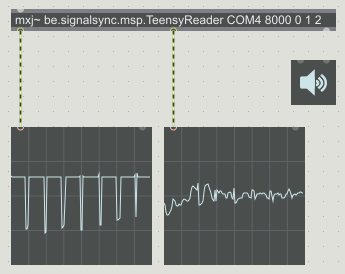
\includegraphics[width=0.4\textwidth]{TeensyReader.png}
	\end{center}
	\label{teensyReader}
\end{figure}

Figuur \ref{teensyReader} toont de TeensyReader waarbij de Teensy samplet aan een frequentie van $8000Hz$. De microfoon is aangesloten op pin A1, de infraroodsensor is aangesloten op pin A0. De links scope module toont het signaal van de infraroodsensor, de rechtse module toont de geluidsgolf.

\subsubsection{Implementatie}

Een Max/MSP module kan in Java geschreven worden door een klasse te laten overerven van \texttt{MSPPerformer}. Bij de constructie worden de \textit{outlets} (de uitgaande verbindingen) geïnitialiseerd en wordt er een \texttt{TeensyDAQ} object aangemaakt. Dit is een object uit afkomstig uit de \texttt{TeensyDAQ} bibliotheek ontwikkeld aan het IPEM. Deze bibliotheek biedt een low-level interface naar de Teensy microcontroller aan. Na het aanmaken van dit object registreert de module zich als \textit{handler}. Om dit mogelijk te maken wordt de methode \texttt{handle} van de interface \texttt{DAQDataHandler} geïmplementeerd. Na het registreren wordt deze methode consequent opgeroepen met samples afkomstig van de Teensy microcontroller. Deze samples worden vervolgens gebufferd.

Een klasse die overerft van \texttt{MSPPerformer} moet de methode \texttt{perform} implementeren. In deze methode worden de samples uit de buffers gehaald, geresamplet naar de Max/MSP samplefrequentie en verstuurd naar de outlets.

\subsection{De synchronisatiemodule}
\label{sync-module}

De tweede module zal de synchronisatie van de streams verzorgen en is geïmplementeerd in de klasse \texttt{Sync}. De module maakt gebruik van \texttt{RealtimeSignalSync} om de latencies tussen de audiostreams te bepalen. De module kan in Max/MSP met volgende code worden aangemaakt: \texttt{mxj\textapprox\  be.signalsync.msp.Sync <<parameter>>}

\subsubsection{Instellen van de stream structuur}

De module verwacht één parameter van het type \texttt{String} die beschrijft hoe de streams gestructureerd zijn. De structuur wordt voorgesteld als een door komma's gescheiden reeks van de letters 'a' en 'd'. Elk door komma's gesplitst deel bepaald de structuur van een \texttt{StreamGroup} waarin de letters 'a' en 'd' respectievelijk voor audiostream en datastream staan. Per deel mag maar eenmaal de letter 'a' voorkomen. De volledige tekenreeks  (de verzameling van alle \texttt{StreamGroups}) stelt de structuur van een \texttt{StreamSet} voor onderverdeeld in \texttt{StreamGroups}.

Dit zou een mogelijke parameter voor deze module kunnen zijn: \texttt{addd,dad}. De eerste \texttt{StreamGroup} bestaat uit 4 streams waarbij de synchronisatie met de eerste stream zal worden uitgevoerd. De tweede \texttt{StreamGroup} bestaat uit 3 streams. De tweede stream stelt hierbij de audiostream voor.

Figuur \ref{maxStreamSync} toont hoe deze module gebruikt moet worden in combinatie met de \texttt{TeensyReader}. De audiostream \textit{outlets} (bepaald door de vierde parameter van de twee \texttt{TeensyReaders}) worden verbonden met de audiostream \textit{inlets} van de \texttt{Sync} module (bepaald door de letters 'a' van de parameter).

\begin{figure}[h!]
	\captionsetup{width=0.8\textwidth}
	\caption[Synchronisatie in Max/MSP]{De synchronisatie van streams in Max/MSP afkomstig van twee Teensy microcontrollers.}
	\begin{center}
		\advance\parskip0.3cm
		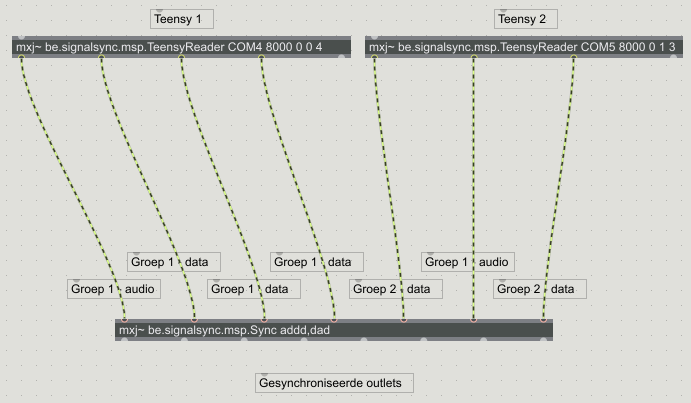
\includegraphics[width=\textwidth]{maxSync.png}
	\end{center}
	\label{maxStreamSync}
\end{figure}

\subsubsection{Implementatie}

Net zoals \texttt{TeensyReader} erft deze module over van \texttt{MSPPerformer}. Ook wordt de interface \texttt{SyncEventListener} geïmplementeerd. In de constructor wordt op basis van de parameter van de module een \texttt{StreamSet} van \texttt{MSPStream} objecten aangemaakt. In de perform methode van de module worden de signaalvectoren doorgegeven aan de \texttt{MSPStream} objecten. De synchronisatie wordt verwezenlijkt door in de constructor een \texttt{RealtimeSignalSync} object aan te maken waarop de klasse zich registreert. Aan het \texttt{RealtimeSignalSync} object wordt de \texttt{StreamSet} meegegeven. Elke keer wanneer er informatie over de latency beschikbaar is wordt de methode \texttt{onSyncEvent} opgeroepen met alle latencies.

Met behulp van deze latencies en de methode beschreven in \ref{corrections} worden de Max/MSP streams gesynchroniseerd.

\subsection{Andere modules}

Aangezien Max/MSP al een groot aantal modules bevat was het niet nodig om bepaalde features in de eigen modules te implementeren. Enkele modules die zeer bruikbaar zijn voor deze toepassing:

\begin{description}
	\item\texttt{sfplay\textapprox} \hfill \\
	Met deze module is het mogelijk om streams van verschillende bestandstypen in te lezen. Dit kan handig zijn om de synchronisatie van een experiment toch als naverwerking uit te voeren.
	
	\item\texttt{sfrecord\textapprox} \hfill \\
	Deze module laat toe om een Max/MSP signaal weg te schrijven naar een bestand. De gesynchroniseerde streams kunnen met behulp van deze module op schijf worden opgeslagen.
	
	\item\texttt{scope\textapprox} \hfill \\
	Deze module toont de golfvorm van een Max/MSP signaal. Dit is handig tijdens het uitvoeren van een experiment om de signalen te controleren.
	
\end{description}


